\subsection{Accessing Memory}

\subsubsection{What is a memory?}

A computer's memory is organized as an array of bytes. Each byte is identified by its address in memory (its position in that array).
\begin{table}[!htp]
    \centering
    \begin{tabular}{@{} c | c @{}}
        \toprule
        Address & Value \\
        \midrule
        \texttt{0x0} & \texttt{16} \\
        \texttt{0x1} & \texttt{255} \\
        \texttt{0x2} & \texttt{14} \\
        \texttt{0x3} & \texttt{0} \\
        \texttt{0x4} & \texttt{0} \\
        \texttt{0x5} & \texttt{0} \\
        \texttt{0x6} & \texttt{6} \\
        \texttt{0x7} & \texttt{0} \\
        \texttt{0x8} & \texttt{32} \\
        \texttt{0x9} & \texttt{48} \\
        \texttt{0xA} & \texttt{255} \\
        \texttt{0xB} & \texttt{255} \\
        \texttt{0xC} & \texttt{255} \\
        \texttt{0xD} & \texttt{0} \\
        \texttt{0xE} & \texttt{0} \\
        \texttt{0xF} & \texttt{0} \\
        \texttt{0x10} & \texttt{128} \\
        \vdots & \vdots \\
        \texttt{0x1F} & \texttt{0} \\
        \bottomrule
    \end{tabular}
    \caption{Example illustration of the program's memory address space of 32 bytes, range from \texttt{0x0} to \texttt{0x1F}.}
\end{table}

\noindent
From the processor's point of view, loading an instruction to access the contents present in memory is done with the \texttt{ld} assembly instruction. For example, \texttt{ld R0 $\leftarrow$ mem[R2]} means \dquotes{take the value from register \texttt{R2} and put that value into register \texttt{R0}}.

\highspace
Before we introduce new concepts, let us take a moment to explain some important \textbf{terminology}:
\begin{itemize}
    \item \definition{Memory Access Latency}, is the \textbf{time} it takes for the \textbf{memory system to deliver data to the processor}.
    
    \item \definition{Processor Stall}. A \textbf{processor} stalls when it \textbf{cannot execute the next instruction in an instruction stream because of a dependency on a previous instruction that has not been completed}. Accessing memory is a major source of stalling, which is one of the main reasons why memory accesses should be limited. 
    \newpage
    For \example{example}, in the following three assembler instructions, the add has to wait for the loading of \texttt{R2} and \texttt{R3} values, making parallelization more complicated:
    \begin{flushleft}
    	\texttt{ld r0 mem[r2]}\newline
    	\texttt{ld r1 mem[r3]}\newline
    	\texttt{add r0, r0, r1}
    \end{flushleft}
    
    \item \definition{Memory Bandwidth}, is the \textbf{rate at which the memory system can provide data to a processor}.

    Bandwidth is the \underline{critical} resource in modern computing.
    
    \textbf{High-performance parallel programs will}:
    \begin{enumerate}
        \item \textbf{Organize computation to fetch data from memory less frequently}. For example, reuse data previously loaded by the same thread (temporal locality optimizations) or share data across threads (inter-thread cooperation);
        
        \item Prefer to \textbf{perform additional arithmetic to store/reload values};
        
        \item \textbf{Programs need to access memory infrequently} to take advantage of modern processors.
    \end{enumerate}
\end{itemize}

\newpage

\subsubsection{How to reduce processor stalls}

\paragraph{Cache}

One of the most common solutions is caching.

\highspace
A \definitionWithSpecificIndex{cache}{Cache}{} is a hardware or software \textbf{component that stores data so that future requests for that data can be served faster}; the data stored in a cache might be the result of an earlier computation or a copy of data stored elsewhere.
\begin{itemize}
    \item A \definition{Cache Hit} occurs when the \textbf{requested data is found} in a cache;
    \item A \definition{Cache Miss} occurs when \textbf{it cannot}.
\end{itemize}
Cache hits are served by reading data from the cache, which is faster than recomputing a result or reading from a slower data store, so the \textbf{more requests that can be served from the cache, the faster the system performs}.\cite{wikipediaCacheResearch}

\highspace
Many modern CPUs have logic that predicts what data will be accessed in the future and \dquotes{pre-fetches} that data into caches. \definition{Prefetching} reduces stalls because the data is resident in the cache when it is accessed. But beware, the other side of the coin is that if the \textbf{guess is wrong}, the \textbf{performance is worse than the system without prefetching}!

\longline

\paragraph{Multi-threading}

A \definition{Multithreaded Processor} is one that has the \textbf{ability to follow multiple instruction streams without software intervention}. In practice, then, this \textbf{includes any machine that stores multiple program counters (PCs) in hardware within the processor} (i.e., on chip, for microprocessor-era machines).\cite{nemirovsky2022multithreading}

\highspace
The main idea in this architecture is to \textbf{interleave processing of multiple threads on the same core to hide stalls}. In other words, if we can't make progress on the current thread, we work on another one.

\begin{examplebox}[: core utilization]\label{example: core utilization}
    To better understand our explanation, suppose we are running a program where threads perform \textbf{three arithmetic instructions followed by a memory load} (with 12 cycle latency).
    \begin{center}
        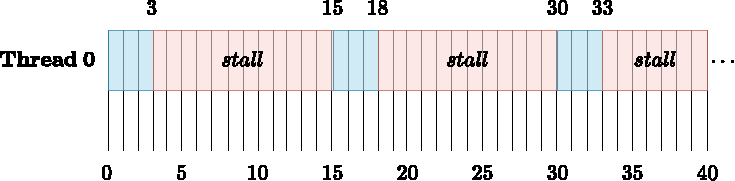
\includegraphics[width=\textwidth]{img/multi-threading-1.pdf}
    \end{center}

    From the figure, it is clear that if we consider an arithmetic instruction and a memory stall, the core is not fully optimized to work at 100\%. In practice, we see that a single arithmetic instruction takes 3 clock cycles and the memory stall takes 12 clock cycles. This means that from this situation we are using the CPU at only 20\% (3 work clock cycles on 15)!

    Without suggesting the final solution, try to see what happens when we add another thread.
    \begin{center}
        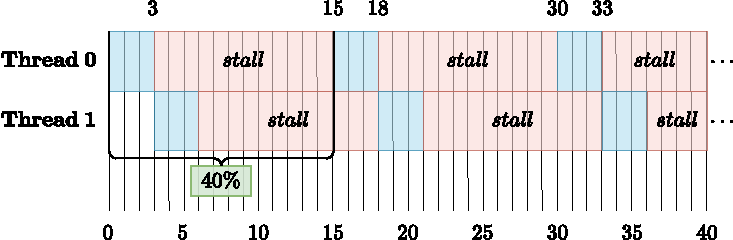
\includegraphics[width=\textwidth]{img/multi-threading-2.pdf}
    \end{center}
    
    We have gained three clock cycles, and now we are taking advantage of the 40\% of the core.

    Now, how many threads do we need to achieve 100\% utilization? The answer is simple: the number of clock cycles of the operations to be done before the stall plus the clock cycles of the stall divided by the working operations (operations that are not stalls). In our case: $15 \div 3 = 5$.
    \begin{center}
        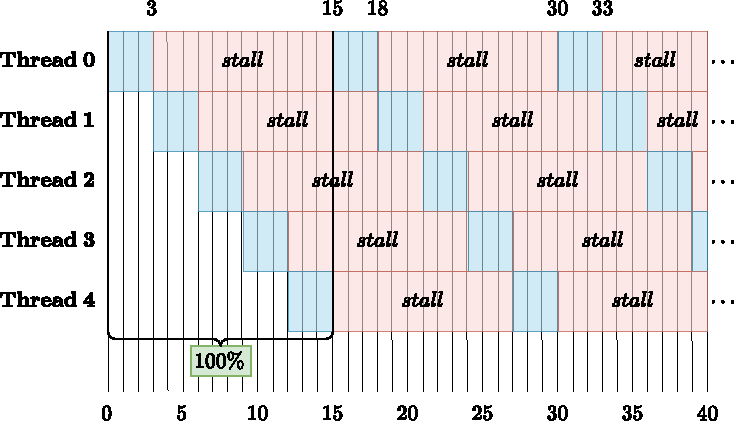
\includegraphics[width=\textwidth]{img/multi-threading-3.pdf}
    \end{center}

    Note that if we add more threads, there will be no benefit because the CPU is already at 100\%.
\end{examplebox}

\begin{flushleft}
    \textcolor{Green3}{\faIcon{check} \textbf{Multithreaded Processor benefits}}
\end{flushleft}
\begin{itemize}
    \item A processor with multiple hardware threads has the \textbf{ability to avoid stalls} by executing instructions from other threads when one thread must wait for a long latency operation to complete. The latency of the memory operation is not changed by multithreading, it just no longer causes reduced processor utilization.
    
    \item A \textbf{multithreaded processor hides memory latency by performing arithmetic from other threads}. Program that feature more arithmetic per memory access need fewer threads to hide memory stalls.
\end{itemize}

\begin{flushleft}
    \textcolor{Red2}{\faIcon{microchip} \textbf{Type of hardware-supported multithreading}}
\end{flushleft}
\begin{itemize}
    \item \textbf{Core manages execution contexts for multiple threads}. This type still has the same number of ALU resources: multi-threading only helps to use them more efficiently in the face of high latency operations such as memory access. The \textbf{processor decides which thread to run each clock cycle}.
    
    \item \definition{Coarse-Grain Multithreading}, also called \blackdefinition{Block Multithreading} or \blackdefinition{Switch-On-Event Multithreading}, has multiple hardware contexts associated  with each processor core. A hardware context is the program counter, register file, and other data required to enabled a software thread to execute on a core. However, only one hardware context has access to the pipeline at a time.\cite{nemirovsky2022multithreading}

    \item \definition{Fine-Grain Multithreading (FGMT)}, also known as \blackdefinition{Interleaved Multithreading} or \blackdefinition{Temporal Multithreading}, is the type just described on the previous pages, as in the example on page \pageref{example: core utilization}.

    \item \definition{Simultaneous Multithreading (SMT)} has multiple hardware contexts associated with each core. In a simultaneous multithreaded processor, instructions from multiple threads are available to be issued on any cycle. Therefore, all hardware contexts, and in particular all register files, must be accessible to the pipeline and its execution resources.\cite{nemirovsky2022multithreading}
    
    In other words, \textbf{each clock}, the \textbf{core selects instructions from multiple threads to execute on ALUs}.
\end{itemize}